\documentclass[a4paper, 12pt]{article}
\usepackage[top=2cm,bottom=2cm,left=2cm,right=2cm,marginparwidth=1.5cm]{geometry}
\usepackage[T2A]{fontenc}
\usepackage{amsmath}
\usepackage{amsfonts}
\usepackage{amsthm}
\usepackage[utf8]{inputenc}
\usepackage[english, russian]{babel}

\usepackage{hyperref}
\usepackage{listings}
\usepackage{multicol}
\usepackage{multirow}
\usepackage{graphicx}
\usepackage{subfigure}
\usepackage{tabularx}
\usepackage{xurl}

\usepackage[backend=biber,style=numeric]{biblatex}
\addbibresource{refs.bib}
\usepackage{csquotes}

\hypersetup{colorlinks=true}

\newtheorem{theorem}{Теорема}
\newtheorem{definition}{Определение}
\newtheorem{corollary}{Следствие}

\title{Применение физически информированного глубокого обучения для решения дифференциальных уравнений}
\author{Даниил Лаптев}

\begin{document}

\maketitle
\tableofcontents

\newpage
\section*{Введение}
\addcontentsline{toc}{section}{Введение}

Дифференциальные уравнения являются одним из ключевых инструментов для описания и анализа окружающего мира. Существует множество способов их классификации согласно каким-либо особенностям формулировки или свойств, которыми обладают решения. Например, они бывают линейными и нелинейными; существует известное деление линейных ДУ в частных производных на гиперболические, параболические и эллиптические; ДУ могут быть детерминированными или стохастическими.

Существует ряд проблем. Во-первых - для некоторых методов, например таких, как конечные разности, конечные элементы и конечные объёмы, существует необходимость выбора подходящего разбиения пространства на соответствующие ячейки, для центров или для узлов которых мы будем вычислять значение искомой функции. Это может быть неприемлемо в некоторых сценариях (например, для моделирования нестатичной геометрии, которая подвержена значительным деформациям или в которой узлы могут исчезать или появляться), или в том случае, когда решение необходимо искать на довольно точной дискретизации ввиду особенностей решения (выраженных нелинейностей, особых точек, шоков, разрывов и прочего) и, кроме того, в случае большого числа переменных это крайне затратно с вычислительной точки зрения - здесь мы наталкиваемся на проклятье размерности. Во-вторых - зоопарк численных методов и относительная сложность их самостоятельной реализации представляет собой ограничение с точки зрения их использования непрофессионалами. Для каждого отдельного случая универсальный, простой метод может не подойти по причине недостаточной точности или неприменимости для решения конкретной задачи; поиск более подходящего, улучшение существующего или выработка нового представляют собой тяжёлое предприятие, которое может отнять много времени.

Использование методов глубокого обучения для таких задач представляет собой перспективное направление, которое в последние годы всё более активно внедряется в науку и технику. Появление методологии Physics-Informed Neural Networks \cite{RAISSI2019686} позволило по-новому взглянуть на то, как можно обучить нейросеть удовлетворять тем или иным законам физики. Технология автоматического дифференцирования позволяет использовать дифференциальные уравнения как один из факторов регуляризации нейросетевой модели - мы внедряем в процесс обучения некоторую априорную информацию, выраженную в форме дифференциальных уравнений, и заставляем нейросетевую модель удовлетворять этим ограничениям. Иными словами, мы информируем нейросетевую модель о том, какие предсказания она должна давать.

В статье \cite{RAISSI2019686} этот подход применён для решения дифференциальных уравнений (прямая задача), а также для идентификации системы - при заданном дифференциальном уравнении и данных о протекании процесса мы решаем задачу обнаружения параметров этого ДУ (обратная задача). Впоследствии эта методология стала применяться для решения различных специфических инженерных задач, краткий обзор которых можно найти в \cite{Cuomo2022} вместе с обзором методологии PINN и её возможных путей развития. В свою очередь экспериментальный и теоретический анализ процесса обучения PINNs для решения дифференциальных уравнений нельзя назвать достаточным, в нём остаются незаполненные пробелы - например, что можно сказать касательно того, как в общем случае связаны краевые задачи, размер нейросетевой модели и гиперпараметры процесса обучения? Как именно алгоритм оптимизации сходится к решению, и каковы условия этой сходимости? Какие существуют особенности процесса обучения PINN, которые заслуживают внимания? И многие другие вопросы.

В данном исследовании будет систематически рассмотрено применение классической методологии PINN для решения ряда различных дифференциальных уравнений, которые отличаются между собой формулировкой, поведением решений, а также сложностью отыскания их решения. В качестве таковых были выбраны простые, но распространённые типы задач - обыкновенное дифференциальное уравнение второго порядка, система ОДУ первого порядка, а также параболическое уравнение в частных производных. Будет предпринята попытка выявить основные принципы работы PINN, основные правила оптимального подбора гиперпараметров, а также обнаружить некоторые особенности тренировки моделей, которые могут представлять интерес с точки зрения теории глубокого обучения или дифференциальных уравнений.

Целью нашего исследования является рассмотрение принципов применения методологии PINN для решения некоторых распространённых типов дифференциальных уравнений (в качестве иллюстративных примеров мы выбрали гармонический осциллятор с затуханием, систему Лотки-Вольтерры и уравнение диффузии), а также выявление того, какую роль играют гиперпараметры нашего сеттинга обучения. Для достижения цели были поставлены следующие задачи:

\begin{enumerate}
    \item Реализовать классические методы для получения решений каждого из рассматриваемых ДУ. Эти решения будут эталонными.
    \item Решить каждую из задач с помощью PINN. Обнаружить, при каких гиперпараметрах решение можно назвать удовлетворительным.
    \item Выявить, как гиперпараметры влияют на решение каждой из задач.
    \item Рассмотреть модели разного размера. Как меняются оптимальные гиперпараметры?
    \item Рассмотреть те же задачи, но с другими параметрами и граничными условиями. Провести анализ влияния гиперпараметров и моделей на качество решения. Осталась ли картина той же, что в пунктах 3 и 4?
    \item Сделать выводы относительно того, как достичь удовлетворительного результата, используя методологию PINN, и можно ли это сделать.
\end{enumerate}

\section{Классическая методология PINNs} \label{section:pinn}

Мы полагаемся на следующую гарантию - почти всякое решение ДУ можно приблизить с произвольной точностью некоторой нейросетевой моделью, если правильно подобрать её архитектуру. В общем случае это утверждение представляется как свойство универсальной аппроксимации \cite{Kratsios2021}. Таким образом, мы больше заинтересованы в процессе приближения решения - достаточно ли экспрессивная модель выбрана, существует ли проблема нехватки информации, затухания градиентов и т.п., насколько хорошие гиперпараметры выбраны, способен ли метод оптимизации эффективно сойтись к минимуму и так далее - нежели в анализе того, какие свойства присущи искомому решению. Может быть, эти свойства прольют свет на какие-то проблемы во время тренировки, или позволят построить нейросетевую модель с определёнными предположениями о решении и тем самым улучшить качество решения, но это является скорее вспомогательным источником информации, нежели необходимым.

Рассмотрим общую постановку PINN. Пусть нам задана некоторая задача с граничными условиями \cite{Cuomo2022}:

\begin{equation*}
\begin{gathered}
    \mathcal{D}[u(z), \gamma] = f(z) \quad z \in \Omega, \\
    \mathcal{B}[u(z)] = g(z) \quad z \in \partial \Omega,
\end{gathered}
\end{equation*}
где элемент $z$ обычно интерпретируется как набор из $D$ пространственных координат и одной временной координаты, т.е. $z = [x_1, ..., x_D, t]^T \in \mathbb{R}^{D + 1}$. Граничные условия также описывают начальные условия при нижней границе $t = 0$. Довольно часто $f(z) \equiv 0$. Дифференциальный оператор $\mathcal{D}$ обычно параметризован набором чисел $\gamma$, который определяет специфический вид ДУ.

Имея некоторую параметризованную функцию $\mathcal{N}(z; \theta)$, мы должны найти такой набор параметров $\theta^*$, что $\mathcal{N}(z; \theta^*) \approx u(z)$ на всём домене $\Omega$.

Методология PINN в сущности представляет собой метод регуляризации процесса обучения нейросетевой модели, при котором мы ограничиваем множество возможных параметров при помощи информации из заданных нами дифференциальных уравнений. Иными словами, множество допустимых параметров $\Theta$ описывается как
$$
\Theta = \{\theta : \quad \mathcal{D}[\mathcal{N}(z; \theta), \gamma] \approx f(z) \quad \text{и} \quad \mathcal{B}[\mathcal{N}(z; \theta)] \approx g(z)\}
$$

Учитывая, что нейросетевые модели редко представляют собой точную аппроксимацию какой-либо функции, мы используем знак $\approx$ вместо $=$, однако понятие близости двух функций очень сильно зависит от конкретной задачи. Возникает следующая ситуация. В реальных условиях, используя нейросетевые аппроксиматоры и ограниченные вычислительные ресурсы, мы не надеемся получить $\mathcal{N}$ такую, что она будет целиком удовлетворять заданным условиям и являться точным выражением $u(z)$ - всегда существует ошибка того или иного рода, которую нам хотелось бы свести к минимуму. В данном случае можем явно выразить интересующую нас ошибку следующим образом. 

Пусть зафиксирована какая-либо архитектура нейросетевой модели, и для неё задан конкретный вектор параметров $\theta \in \mathbb{R}^p$. Тогда качество нейросетевой аппроксимации мы определяем как
\begin{equation} \label{eq:pinn:losses}
    \begin{aligned}
    \mathcal{L}_D(\theta) &= \int_{\Omega} \|\mathcal{D}[\mathcal{N}(z; \theta), \gamma] - f(z)\|dz  \\
    \mathcal{L}_B(\theta) &= \int_{\partial \Omega}\|\mathcal{B}[\mathcal{N}(z; \theta)] - g(z)\|dz
    \end{aligned}
\end{equation}

На практике эти величины можно оценить методом Монте-Карло, а в качестве нормы выбрать квадрат Евклидовой нормы - тогда мы получим метрику Mean Squared Error, используемую нами в качестве функции потерь для оптимизации нейросетевой модели.

Функции ошибки $\mathcal{L}_D$ и $\mathcal{L}_B$ позволяют оценить, насколько хорошо нейросетевая модель удовлетворяет постановке краевой задачи. Мы ожидаем, что модель, минимизирующая обе функции ошибки, тем самым аппроксимирует решение. Более того, в некоторых случаях мы даже обладаем гарантиями сходимости (см. например \cite{vandermeer2021optimally}, теорема 1).

Сформулируем полную функцию ошибки. На границе мы выбираем пары $\{z_i, u(z_i)\}$, исходя из постановки задачи, а в области $\Omega$ мы выбираем произвольные точки $\{z_j\}$. Пусть количество выбранных точек на границе будет $N_\mathcal{B}$, внутри области - $N_\mathcal{D}$. Тогда в качестве функции ошибки можно использовать взвешенную сумму ошибок внутри области $\Omega$ и на её границе:
\begin{equation} \label{eq:pinn:empiricalLoss}
\mathcal{L}(\theta) = \frac{\alpha}{N_\mathcal{B}} \sum_{i = 1}^{N_\mathcal{B}} (\mathcal{B}[\mathcal{N}(z_i; \theta)] - u(z_i))^2 + \frac{\beta}{N_\mathcal{D}} \sum_{j = 1}^{N_\mathcal{D}} (\mathcal{D}[\mathcal{N}(z_j; \theta), \gamma] - f(z_j))^2
\end{equation}

Отметим, что до сих пор мы обходимся без каких-либо данных, кроме тех, которые являются частью постановки краевой задачи. В стандартном сеттинге обучения с учителем мы обладаем информацией о значениях искомой функции в некоторых точках - чем её больше, тем лучше. В текущем сеттинге мы обладаем лишь информацией о том, какие значения принимает искомая функция (и/или её производные) на границах заданного домена $\Omega$. Кроме того, мы можем получить приближённое решение, даже не имея явно заданной функции на границе, а только набор её измерений - это мы рассмотрим далее. Если вдруг у нас имеется набор значений искомой функции, мы можем добавить ещё один терм функции потерь.

В конечном итоге для какой-либо фиксированной нейросетевой архитектуры мы ищем такой набор параметров $\theta^*$, что
$$
\theta^* = \arg \min_{\theta} \mathcal{L}(\theta)
$$

В качестве нейросетевой архитектуры мы используем модели прямого распространения (FF), которые представляются как композиция аффинных и нелинейных преобразований:
\begin{equation} \label{eq:pinn:networkArchitecture}
    \begin{gathered}
        Linear_i(x) = W_ix + b_i,\\
        FF(z) = Linear_L(...\nu(Linear_1(z))),
    \end{gathered}
\end{equation}
где $\nu$ - некая нелинейная функция, в нашем случае - гиперболический тангенс.

Для наших экспериментов мы возьмём такие модели, у которых количество строк в матрицах $W_1, ..., W_{L-1}$ одинаково. Пусть это количество (ширина нейросети) записывается как $W$. Тогда модель глубины $L$ и ширины $W$ будет обозначаться как $\mathrm{FF}_{L, W}$.

\section{Решение дифференциальных уравнений} \label{section:diffeqsolving}

\subsection{Гармонический осциллятор с затуханием}

На данный момент нас не интересуют её физические свойства, только математическая формулировка. Система описывается следующим образом:
\begin{equation} \label{eq:oscillator:diffeq}
    \frac{\mathrm{d}^2 x}{\mathrm{d} t^2} + 2\zeta \omega_0\frac {\mathrm {d} x}{\mathrm {d} t} + \omega _0^2x = 0,
\end{equation}
где функция $x(t) : \mathbb{R} \to \mathbb{R}$ описывает положение осциллирующей массы, а параметры $\zeta$ и $\omega$ влияют на характер затухания осцилляции.

Пусть дано начальное положение массы $x(0) = x_0$ и начальная скорость $v(0) = \frac{\mathrm{d} x}{\mathrm{d} t}(0) = v_0$. Зафиксируем некоторую нейросетевую архитектуру $\mathcal{N}(z; \theta)$. Тогда мы должны отыскать такие параметры $\theta$, которые минимизируют следующий функционал:
\begin{equation*}
    \mathcal{L}(\theta) = \frac{\alpha}{2}((\mathcal{N}(0; \theta) - x_0)^2 + (\frac{\mathrm{d}\mathcal{N}}{\mathrm{d}t}(0; \theta) - v_0)^2) + \frac{\beta}{N_{\mathcal{D}}} \sum_{i = 1}^{N_{\mathcal{D}}} \Big(\Big[\frac{\mathrm{d}^2}{\mathrm{d} t^2} + 2\zeta \omega_0\frac {\mathrm {d}}{\mathrm {d} t} + \omega _0^2\Big]\mathcal{N}(t_i; \theta)\Big)^2
\end{equation*}

Мы ожидаем, что при достаточно хорошем выборе модели, алгоритма оптимизации и гиперпараметров наша нейросетевая модель будет аппроксимировать функцию решения $\hat{x}(t)$. В качестве ориентира возьмём решение методом Рунге-Кутты с помощью пакета Scipy, и будем считать метрику
$$
\mathrm{RMSE}(\theta) = \sqrt{\frac{1}{128}\sum_{i=1}^{128}(\mathcal{N}(t_i;\theta) - \mathrm{RK4}_i)^2},
$$
где $t_i$ расположены равномерно на интервале $\Omega = [0, T]$.

Пусть дифференциальное уравнение \ref{eq:oscillator:diffeq} задано с параметрами $\zeta = 0.2$, $\omega_0 = 2.0$, и начальное условие задано как $x_0 = 5$, $v_0 = 7$. Интересующая нас область $\Omega = [0, 10]$. На рис. \ref{fig:oscillator:solution} приведён результат обучения модели $\mathrm{FF}_{2, 32}$ после 10000 итераций с использованием оптимизатора Adam.

\begin{figure}
    \centering
    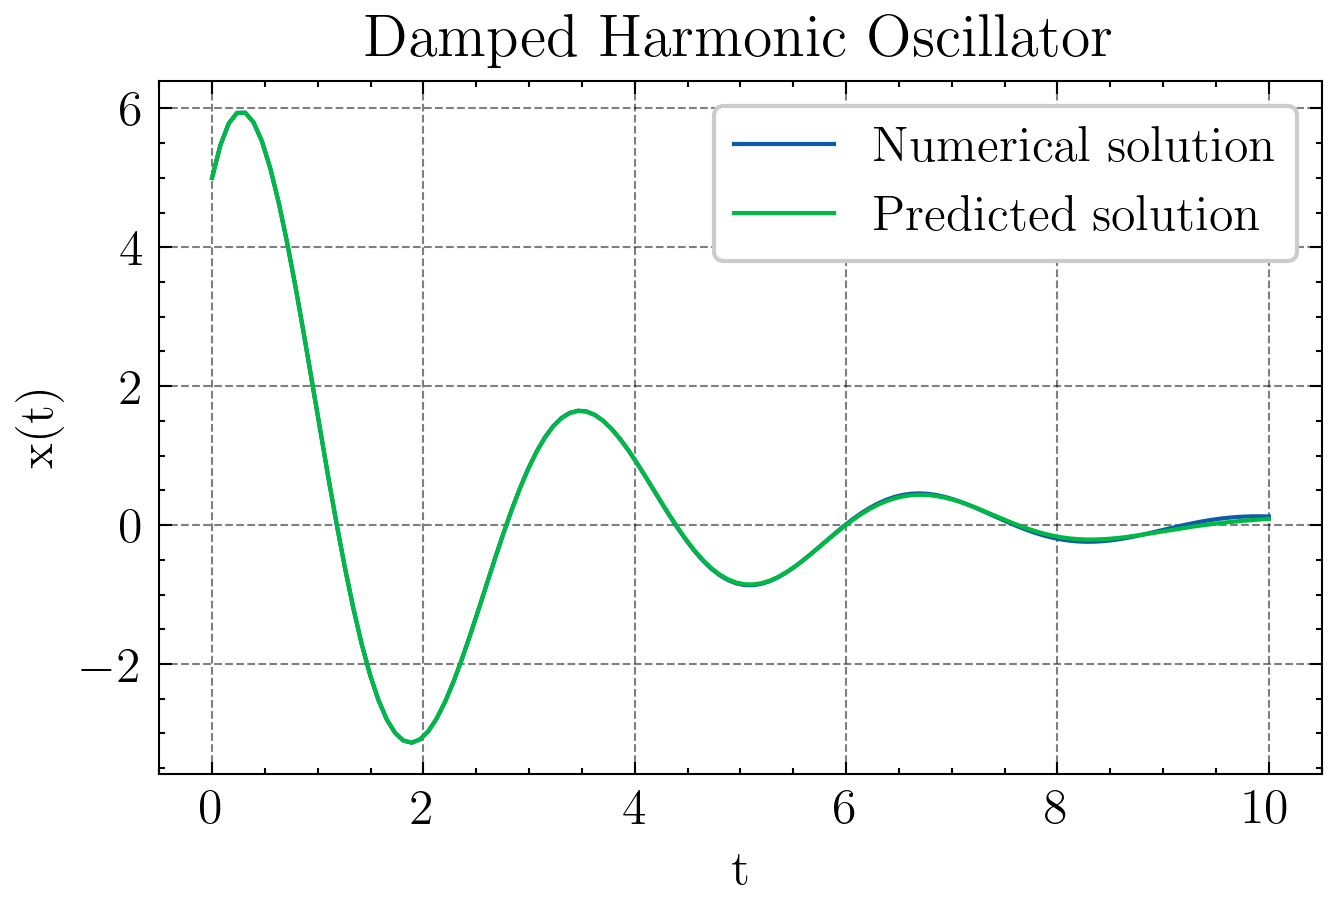
\includegraphics{../images/oscillator/Damped Harmonic Oscillator.png}
    \caption{Сравнение численного решения с предсказаниями PINN после 10000 итераций обучения. Гиперпараметры были выбраны следующие: $N_\mathcal{D} = 256$, $\alpha = 1$, $\beta = 0.5$, $\mathrm{lr} = 0.001$. Видно, что к концу отрезка точность начинает падать.}
    \label{fig:oscillator:solution}
\end{figure}

\subsection{Система Лотки-Вольтерры}

Теперь рассмотрим модель взаимодействия двух биологических видов, один из которых выполняет роль хищника, другой - жертвы. Такая система часто моделируется с помощью стандартной системы Лотки-Вольтерры. Пусть число особей в их популяциях описывается, соответственно, $y(t)$ и $x(t)$, которые являются непрерывными функциями. Тогда динамика числа особей может быть выражена с помощью системы ОДУ первого порядка
\begin{equation} \label{eq:lotkavolterra:diffeq}
\begin{cases}
    \frac{\mathrm{d}x}{\mathrm{d}t} = \alpha x - \beta x y \\
    \frac{\mathrm{d}y}{\mathrm{d}t} = \delta y x - \gamma y
\end{cases},
\end{equation}
где параметры $\alpha, \beta, \delta, \gamma$ характеризуют рождаемость и смертность популяций.

Как применить методологию PINN, если здесь функции решения две, а не одна?

\paragraph{Подход первый.} Мы можем аппроксимировать функции $x(t)$ и $y(t)$ соответственно двумя нейросетевыми моделями; можно попытаться обучать их одновременно. Однако масштабируемость такого подхода сомнительна - что, если нам потребуется работать с подобного рода системами значительно большего размера, например, в области молекулярной динамики? Тем не менее, для небольшого числа функций этот способ может быть удовлетворительным.

Пусть нейросетевые модели $\mathcal{X} = \mathcal{X}(t; \theta_x)$ и $\mathcal{Y} = \mathcal{Y}(t; \theta_y)$ соответственно приближают функции решения. Пусть даны начальные значения $x_0, y_0$. Нам необходимо найти такие параметры $\theta_x, \theta_y$, которые минимизируют следующие функции ошибки:
\begin{equation} \label{eq:lotkavolterra:losses}
\begin{gathered}
    \mathcal{L_I} = \frac{1}{2}((\mathcal{X}(0) - x_0)^2 + (\mathcal{Y}(0) - y_0)^2) \\
    \mathcal{L_X}(\theta_x, \theta_y) = \frac{1}{N_\mathcal{D}} \sum_{i=1}^{N_\mathcal{D}} \Big(\frac{\mathrm{d}\mathcal{X}}{\mathrm{d}t}(t_i)  - \alpha\mathcal{X}(t_i) + \beta\mathcal{X}(t_i)\mathcal{Y}(t_i)\Big)^2 \\
    \mathcal{L_Y}(\theta_x, \theta_y) = \frac{1}{N_\mathcal{D}} \sum_{i=1}^{N_\mathcal{D}} \Big(\frac{\mathrm{d}\mathcal{Y}}{\mathrm{d}t}(t_i) - \delta\mathcal{X}(t_i)\mathcal{Y}(t_i) + \gamma\mathcal{Y}(t_i)\Big)^2
\end{gathered}
\end{equation}

В качестве итоговой функции потерь мы возьмём их линейную комбинацию:
$$
\mathcal{L_T} = w_1\mathcal{L_I} + w_2\mathcal{L_X} + w_3\mathcal{L_Y}
$$

Пусть дано количество особей в начальный момент времени $x(0) = 10$, $y(0) = 5$, и мы хотим рассмотреть динамику популяций на отрезке $\Omega = [0, 25]$. Параметры нашей модели таковы: $\alpha = 0.4$, $\beta = 0.1$, $\delta = 0.1$, $\gamma = 0.6$. В качестве нейросетевых моделей мы используем $\mathrm{FF}_{1,32}$. Решение, полученное после 50000 итераций, представлено на рисунке \ref{fig:lotkavolterra:first:solution}. Параметры каждой из нейросетей обновляются по отдельности с использованием алгоритма Adam.

Как мы выяснили из данных о протекании процесса обучения, увеличение количества итераций почти всегда приводит к лучшему результату. Иными словами, мы не встречали переобучение - скорее, необходимо подбирать подходящий learning rate, чтобы он одновременно позволил быстро сойтись к минимуму и не выпрыгивал из него.

\begin{figure}
    \centering
    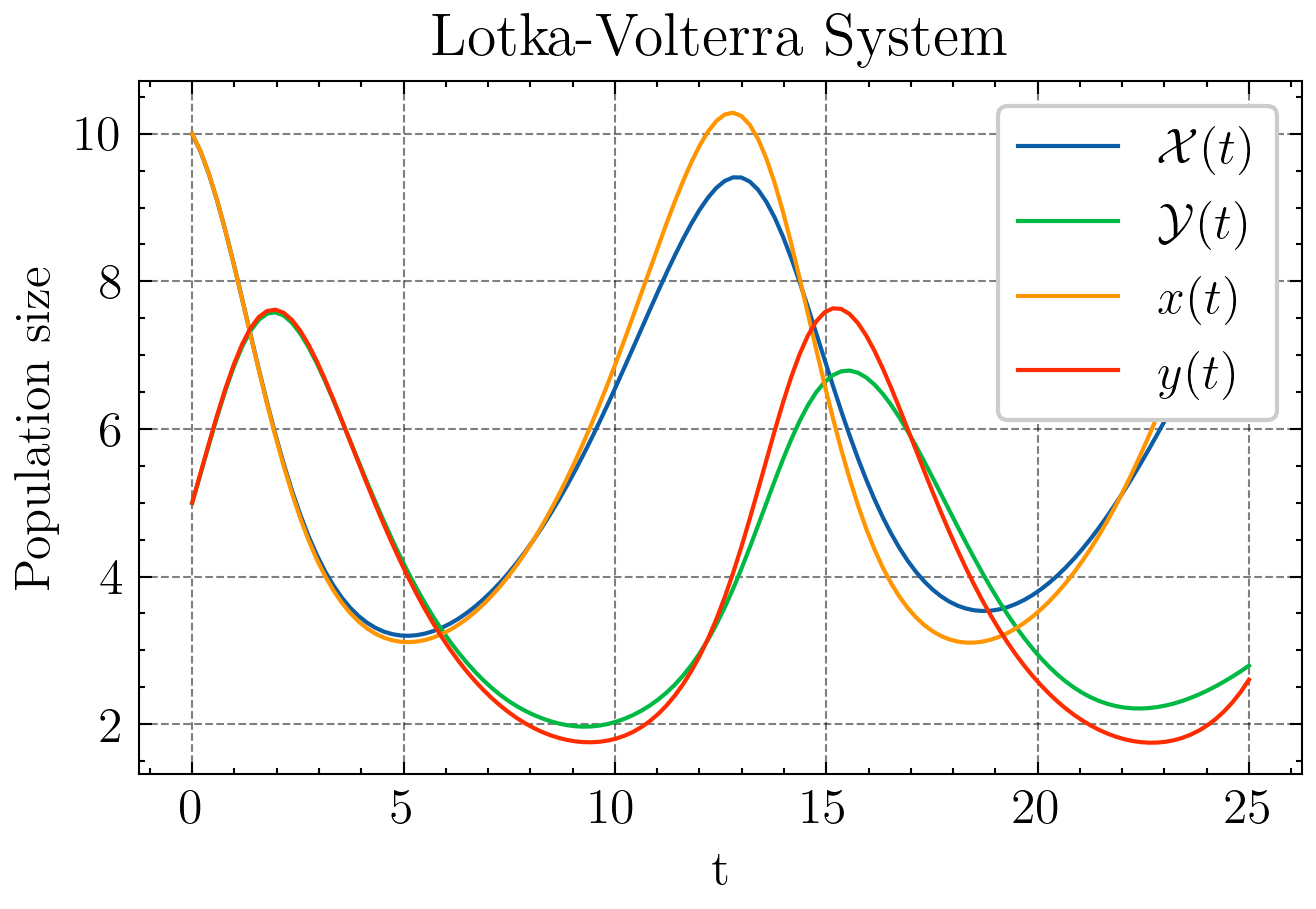
\includegraphics{../images/lotkavolterra/first approach/Lotka-Volterra System.png}
    \caption{Сравнение численного решения системы с полученным нейросетевым решением. Гиперпараметры были выбраны следующие: $w_1 = 1$, $w_2 = w_3 = 2$, $N_\mathcal{D} = 1024$ и $\mathrm{lr} = 0.01$.}
    \label{fig:lotkavolterra:first:solution}
\end{figure}

В результате проведения экспериментов было выяснено, что этот подход довольно чувствителен к инициализации нейросетевой модели - в некоторых случаях обучение упиралось в RMSE $\approx 5$ для $x(t)$ и $\approx 3.2$ для $y(t)$. Это было связано с тем, что нейросетевые модели примерно на $[0, 5]$ научились аппроксимировать решение, а на оставшейся части домена они аппроксимировали нулевую функцию. Мы обнаружили, что инициализация из равномерного распределения на [0, 1) является более надёжной и в среднем даёт лучший результат, чем другие способы (Xavier Uniform, Normal, Kaiming Uniform, Constant), несмотря на то, что обычно в литературе по обучению PINNs используют инициализацию Xavier Uniform \cite{rathore2024challenges}, \cite{wang2020pinns}. Кроме того, в статье \cite{Pang_2019} проводится более подробный анализ методов инициализации нейросетевых моделей и их влияния на сходимость процедуры обучения.

Наиболее интересным нам показалось разделение процесса обучения на фазы. В одном из запусков мы наблюдали следующую картину (рисунок \ref{fig:lotkavolterra:first:losses}). Примерно на 12000 итерации происходит заметное изменение среднего значения RMSE, а также значений функций потерь; несмотря на то, что абсолютные величины здесь достаточно малы, смена фазы легко наблюдаема. Перед этим изменением видно некоторое торможение обучения - значения ошибок изменяются всё меньше, и можно сказать, что мы будто бы выходим на плато. На второй фазе динамика функций потерь становится более выраженной.

\begin{figure}
    \centering
    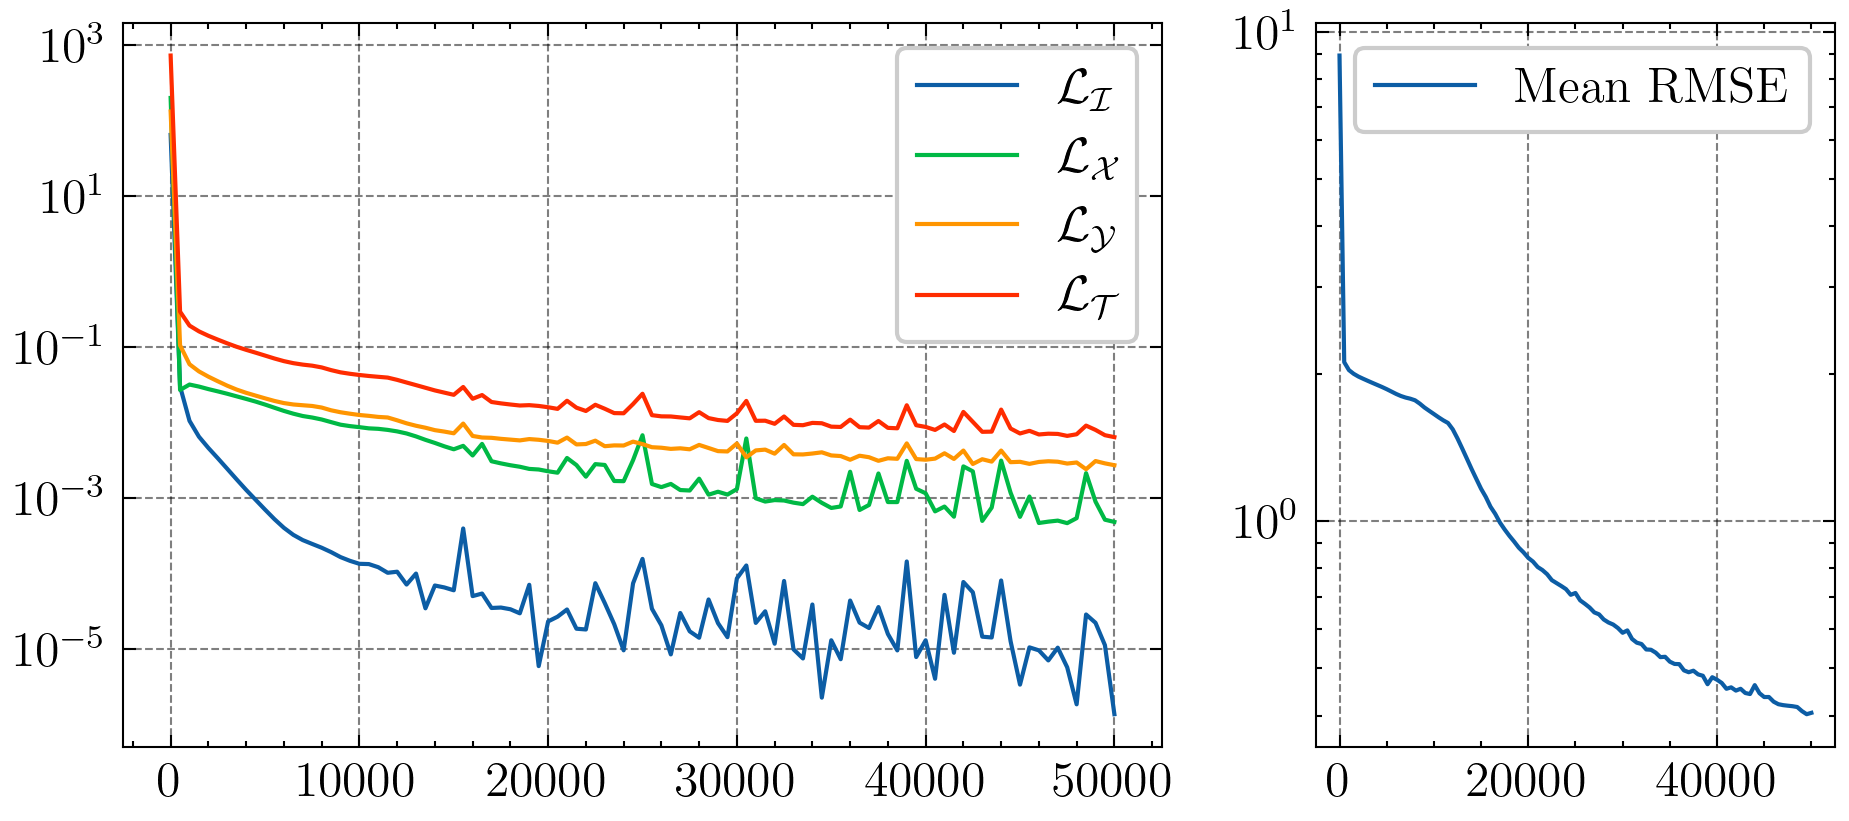
\includegraphics{../images/lotkavolterra/first approach/Losses.png}
    \caption{Изменение значения функций ошибок в процессе обучения. Видно, что примерно на 12000 итерации происходит изменение фазы обучения. Появление этого перехода зависит от инициализации нейросетевых моделей, случайных направлений обучения оптимизатора и, может быть, каких-то других факторов.}
    \label{fig:lotkavolterra:first:losses}
\end{figure}

Наши наблюдения показывают, что этим фазам соответствует обучение различным особенностям искомых функций. Во всех запусках первая фаза соответствует аппроксимации примерно в области [0, 5], причём в остальной области нейросетевые модели выглядят как прямые. Обычно она заканчивается около 10000 итерации. На второй фазе происходит аппроксимация в оставшейся части домена (вместе с дообучением на [0, 5], которое, однако, гораздо менее выражено). Здесь нейросетевые модели начинают повторять форму искомых функций. В некоторых запусках было визуально заметно, что нейросетевые аппроксимации будто бы смещены вправо по горизонтали относительно искомых функций, и третьей фазой в таком случае иногда являлось устранение этого смещения.

Исследование этого феномена мы оставим на будущее, поскольку для этого потребуется анализировать то, как оптимизатор выбирает направление движения, а также рассматривать ландшафт потерь и его свойства. Пока что его можно связать с тем, что, грубо говоря, существуют области, ответственные за те или иные особенности аппроксимации - например, на первой фазе обучения оптимизатор находился в области, <<где аппроксимируется значение функции от 0 до 5>>; на второй фазе он двигался в области, <<в которой повторяется кривизна искомых функций>>; на третьей фазе он перешёл в область <<горизонтального смещения>>. Названия, конечно, совершенно произвольные, однако это может оказаться продуктивным способом рассмотрения процесса обучения PINNs.

\paragraph{Второй подход.} Мы аппроксимируем $u(t) = \{x(t), y(t)\} : \mathbb{R} \to \mathbb{R}^2$. Это выглядит гораздо более эффективным подходом в случае большого числа искомых функций, поскольку достаточно всего лишь изменить количество выходов нейросети.

В данном случае мы снова минимизируем \ref{eq:lotkavolterra:losses}, только теперь используя всего одну нейросетевую модель. Результат после 30000 итераций с использованием модели $\mathrm{FF}_{2, 64}$ представлен на рисунке \ref{fig:lotkavolterra:second:solution}.

\begin{figure}
    \centering
    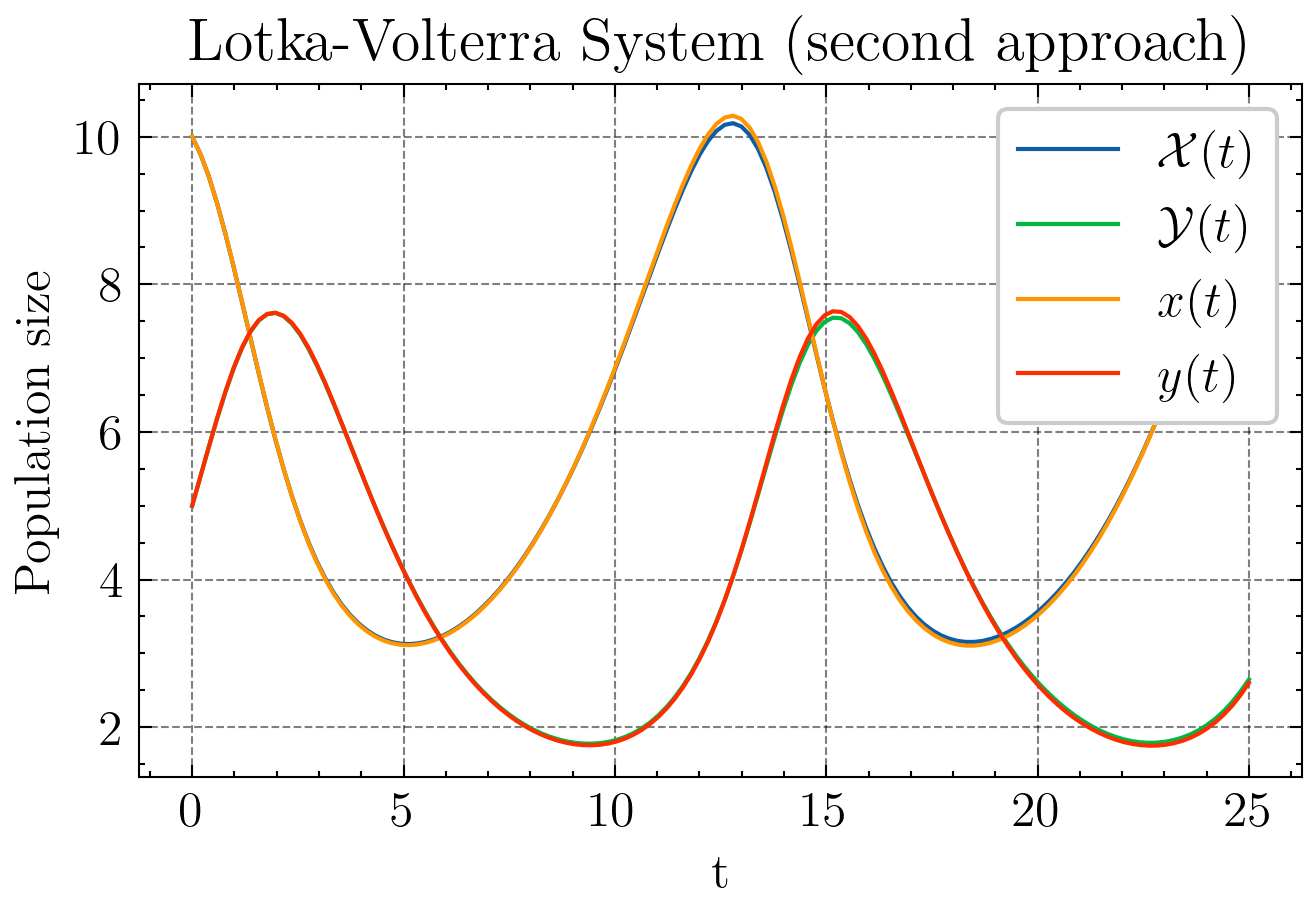
\includegraphics{../images/lotkavolterra/second approach/Lotka-Volterra System (second approach).png}
    \caption{Результат, полученный с использованием второго подхода. Гиперпараметры выбраны следующие: $N_\mathcal{D} = 1024$, $w_1 = 1$, $w_2 = w_3 = 2$, $\mathrm{lr} = 0.001$.}
    \label{fig:lotkavolterra:second:solution}
\end{figure}

Эксперименты показали, что данный подход требует для себя меньших вычислительных ресурсов (так как используется всего один оптимизатор и всего одна модель, вместо двух в предыдущем случае) и вместе с этим позволяет достичь лучшего результата за меньшее число итераций, при условии удачной инициализации. В данном случае наилучшим образом себя показала инициализация Normal (0, 1), хоть и нечасто удавалось получить качественный старт. Инициализация Uniform (0, 1), которая использовалась в предыдущем варианте, приводила к аппроксимации прямой.

Обучение этой модели проходит более равномерно (рисунок \ref{fig:lotkavolterra:second:losses}). Разделить процесс на фазы здесь можно лишь условно. Можно сделать вывод, что в данном случае ландшафт функции потерь гораздо более гладкий, чем при использовании первого подхода, или что оптимизатору становится гораздо легче обнаружить подходящее направление движения. Анализ этого процесса мы оставим на отдельную работу.

\begin{figure}[h]
    \centering
    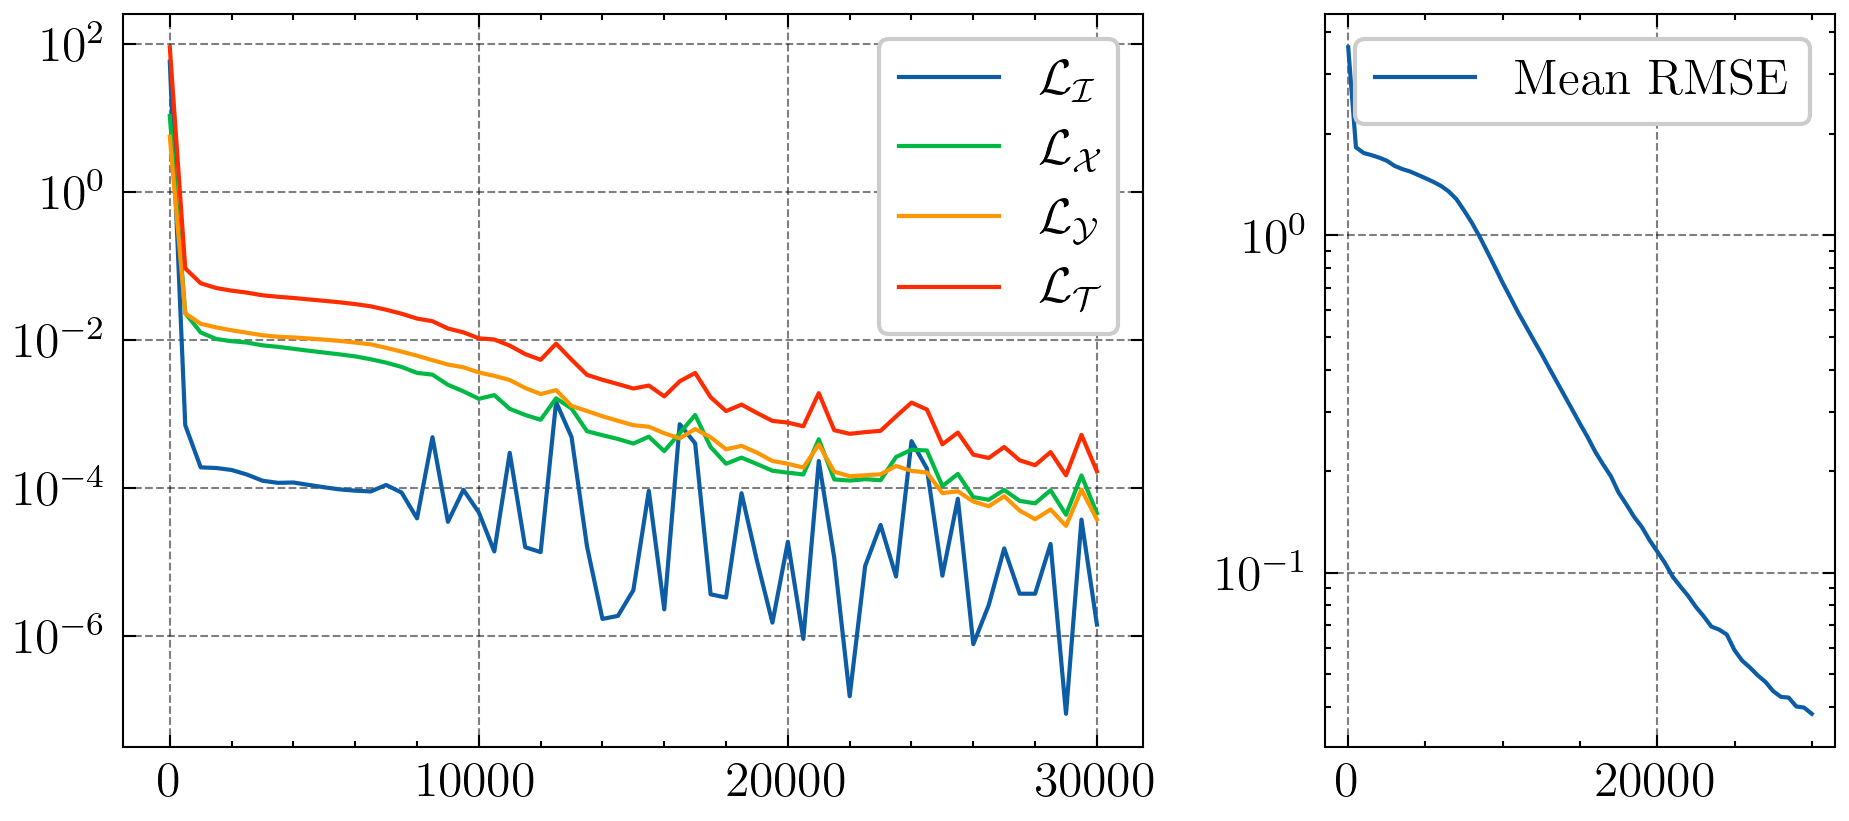
\includegraphics{../images/lotkavolterra/second approach/Losses.png}
    \caption{Динамика функций ошибок во втором подходе.}
    \label{fig:lotkavolterra:second:losses}
\end{figure}

Имеет смысл также отметить, что с течением времени ландшафт потерь усложняется и оптимизатору становится сложнее выбрать направление движения - это заметно по растущим колебаниям функций потерь. Несмотря на то, что RMSE падает вполне равномерно и быстро, в какой-то момент мы можем столкнуться с необходимостью подбирать меньшую величину learning rate. 

В литературе, между тем, нередко используют комбинацию оптимизаторов Adam и L-BFGS или исключительно L-BFGS \cite{Cuomo2022}, \cite{RAISSI2019686}, тогда как в наших экспериментах мы ограничились использованием алгоритма Adam.

% \paragraph{Третий подход.} Мы можем рассматривать аппроксимацию не самого решения, а правила изменения состояния системы. Пусть состояние системы в момент $i$ задано вектором $\mathbf{x}_i \in R^n$. Тогда следующее состояние системы может быть выражено, например, одним из следующих способов:
% \begin{equation*}
% \begin{aligned}
% \mathbf{x}_{i+1} &= \mathcal{F}(\mathbf{x}_i, \mathcal{N}(\mathbf{x}_i; \theta)\\
% \mathbf{x}_{i+1} &= \mathbf{x}_i + \mathcal{N}(\mathbf{x}_i; \theta)\\
% \mathbf{x}_{i+1} &= \mathbf{x}_i + h(\mathbf{x}_i, i)\mathcal{N}(\mathbf{x}_i; \theta)
% \end{aligned}
% \end{equation*}

% В данном случае мы близко подбираемся к идее NeuralODE \cite{chen2019neural} и использования (или имитации) различных методов интегрирования по времени. Его можно рассматривать как один из возможных вариантов применения PINN для моделирования динамических систем, в которых нас интересует дискретная динамика. Подобный подход был эффективно использован для решения уравнения Аллена-Кана в работе \cite{RAISSI2019686}.

% Пусть мы решаем задачу с начальными знаачениями для вектор-функции $u(x, t)$:
% $$
% \frac{\mathrm{d}u}{\mathrm{d}t} = f(x, t, u); \quad u(x, 0) = u_0
% $$

% Тогда для решения этой задачи можно воспользоваться методами Рунге-Кутты. Пусть дан векторы коэффициентов $\mathbf{c}$, $\mathbf{b}$, $\mathbf{b}^*$ и матрица $\mathbf{A}$, которые определяют специфический метод из этого семейства.

\subsection{Уравнение диффузии}

Эта модель используется как самостоятельное описание процесса диффузии или как особый случай некоторых других моделей. Мы рассмотрим одномерный случай и задачу с граничными условиями.

Пусть имеется функция $u(\mathbf{x}, t) : \mathbb{R}^{N + 1} \to \mathbb{R}$, которая описывает, например, концентрацию вещества в какой-либо точке пространства и времени (в нашем случае $N = 1$). Пусть число $D$, называемое коэффициентом диффузии, является постоянным на всей ограниченной области $[A, B] \times [0, T]$. Кроме того, на границах этой области нам известно поведение искомой функции. Тогда краевую задачу для уравнения диффузии мы запишем как
\begin{equation} \label{eq:diffusion:problemStatement}
\begin{gathered}
    \frac{\partial u}{\partial t} = D \frac{\partial^2 u}{\partial x^2}, \\
    u(x, 0) = f(x), \\
    u(A, t) = g_1(t), \\
    u(B, t) = g_2(t),
\end{gathered}
\end{equation}
причём вместо функций на границах мы можем иметь лишь некоторый набор измерений.

Пусть при $t = 0$ и на границах выбирается соответственно $N_I$, $N_A$, $N_B$ точек вместе с заданными в них значениями искомой функции. Внутри области мы берём $N_D$ произвольных точек. Тогда функции потерь мы можем записать как
\begin{equation} \label{eq:diffusion:loss}
\begin{gathered}
    \mathcal{L_I} = \frac{1}{N_I}\sum_{i=1}^{N_I} (\mathcal{N}(x_i, 0) - f(x_i))^2,\\
    \mathcal{L_B} = \frac{1}{N_A}\sum_{i=1}^{N_A} (\mathcal{N}(A, t_i) - g_1(t_i))^2 + \frac{1}{N_B}\sum_{i=1}^{N_B} (\mathcal{N}(B, t_i) - g_2(t_i))^2,\\
    \mathcal{L_D} = \frac{1}{N_D}\sum_{i=1}^{N_D} \Big(\frac{\partial \mathcal{N}}{\partial t}(x_i, t_i) - D \frac{\partial^2 \mathcal{N}}{\partial x^2}(x_i, t_i)\Big)^2
\end{gathered}
\end{equation}

В качестве упрощения мы рассмотрим задачу на области $[0, 1] \times [0, 0.5]$, где коэффициент диффузии $D = 0.7$ и на границах заданы условия:
$$
f(x) = \sin(2 \pi x)^2, \quad g_1(t) = 0, \quad g_2(t) = 0
$$

\begin{figure}
    \centering
    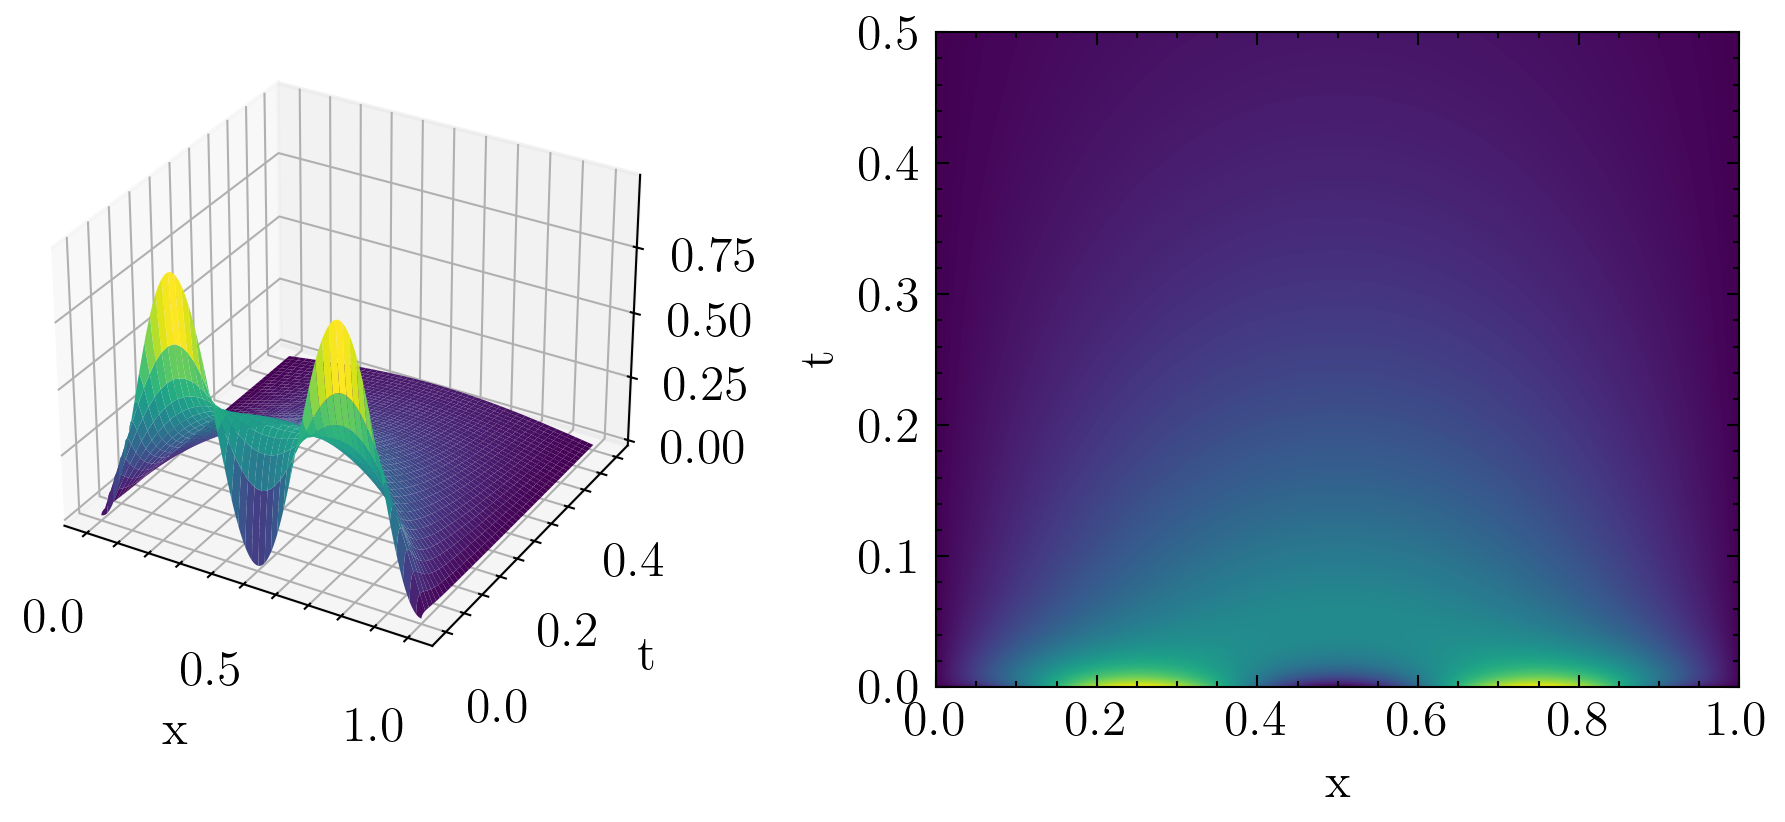
\includegraphics{../images/diffusion/Numerical solution.png}
    \caption{Численное решение краевой задачи \ref{eq:diffusion:problemStatement}. Мы взяли 1000 шагов по времени и 250 шагов по пространству (т.о. $\Delta t = 0.0005$ и $\Delta x = 0.004$). Детали реализации см. в приложении \ref{section:appendix:pinn}.}
    \label{fig:diffusion:numerical}
\end{figure}

Численное решение, полученное с использованием метода Кранка-Николсона, представлено на рисунке \ref{fig:diffusion:numerical}. 

Вместо того, чтобы считать просто взвешенную сумму термов функции потерь, мы выбираем коэффициент $\alpha \in (0, 1)$ и вычисляем сумму следующего вида:
$$
\mathcal{L_T} = \alpha (\mathcal{L_I} + \mathcal{L_B}) + (1 - \alpha) \mathcal{L_D}.
$$

Гипотетически, это позволяет нам балансировать между качеством аппроксимации на границе и внутри домена. Этот подход вдохновлён работой \cite{vandermeer2021optimally}, в которой даются теоретические оценки оптимального выбора коэффициента $\alpha$.

Мы обучили $\mathrm{FF}_{2, 32}$ на 10000 итерациях с $\mathrm{lr} = 0.003$ и достигли итогового значения в $\mathrm{RMSE} = 0.00514$. Точки на границах выбирались случайным образом - при $t = 0$ было взято 128 точек, а при $x = A$ и $x = B$ было взято по 64 случайные точки. Внутри области мы брали 2048 точек, взятых из равномерного распределения на $[A, B] \times [0, T]$. В нашем случае коэффиент $\alpha$ мы взяли равным $0.8$. 

График абсолютного значения разницы между численным решением и нейросетевым представлен на рисунке \ref{fig:diffusion:error}. Видно, что на границе существуют точки, в которых функция решения аппроксимирована достаточно хорошо, тогда как на остальных граничных точках предсказания нейросети начинают отклоняться. Это можно связать с тем, как были выбраны точки коллокации. Мы наталкиваемся на стандартный факт из области машинного обучения - чем больше мы выбираем точек, и чем лучше мы можем ими выразить форму искомой функции (например, сконцентрировав их там, где изменения функции заметны сильнее всего, и уменьшив их концентрацию там, где функция практически не изменяет своей кривизны), тем лучше сможет нейросетевая модель аппроксимировать решение. Тем самым основной задачей, как и во всём машинном обучении, становится сбор наиболее подходящих данных для обучения.

\begin{figure}[h]
    \centering
    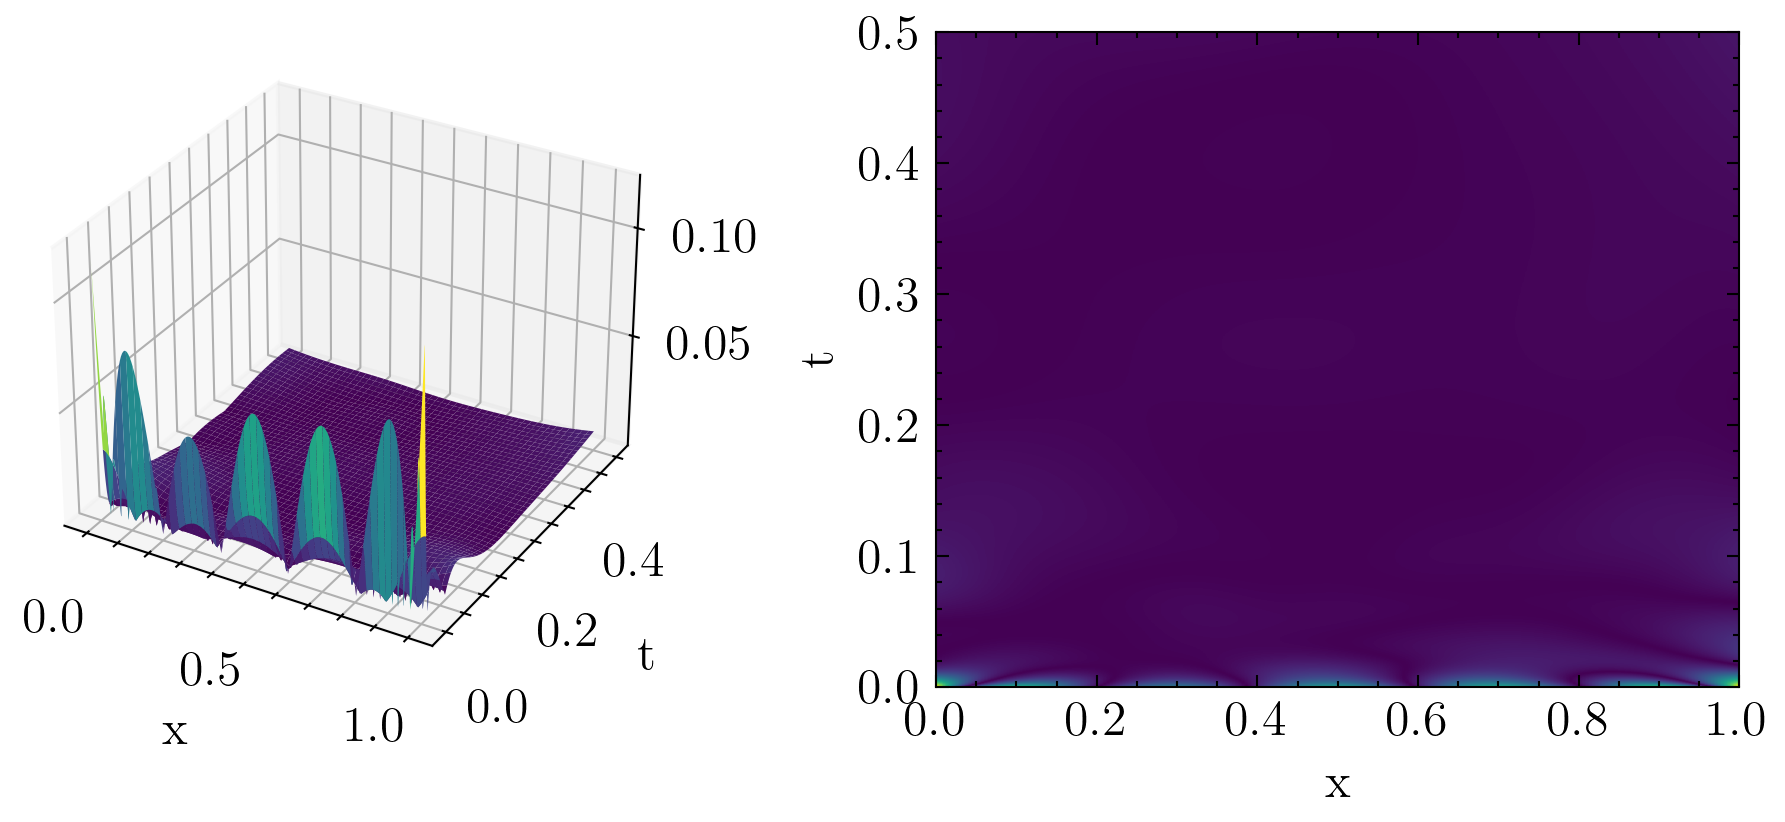
\includegraphics{../images/diffusion/Error.png}
    \caption{Абсолютная величина разницы между численным решением и предсказаниями модели. Неравномерность ошибок связана в первую очередь с тем, как были распределены случайно выбранные точки коллокации.}
    \label{fig:diffusion:error}
\end{figure}

На рисунке \ref{fig:diffusion:losses} представлены значения фунций ошибок в процессе тренировки. Здесь также можно увидеть разделение на фазы - с одной стороны, оно видно по динамике функций ошибок, а с другой стороны его можно заметить, взглянув на анимацию обучения нейросетевой модели\footnote{Анимация доступна по следующей ссылке: \url{https://github.com/DaniilLaptev/Coursework/blob/main/images/diffusion/learning.gif}, и, кроме того, этот эффект легко воспроизводим при указанном нами сеттинге обучения.}. За 2500 итераций нейросеть обучилась аппроксимировать такое решение, как если бы его значения при $t=0$ задавались функцией $\sin(\pi x)$. Затем нейросеть стала постепенно разделять значение в нуле на две вершины и аппроксимировать заданное начальное условие.

\begin{figure}
    \centering
    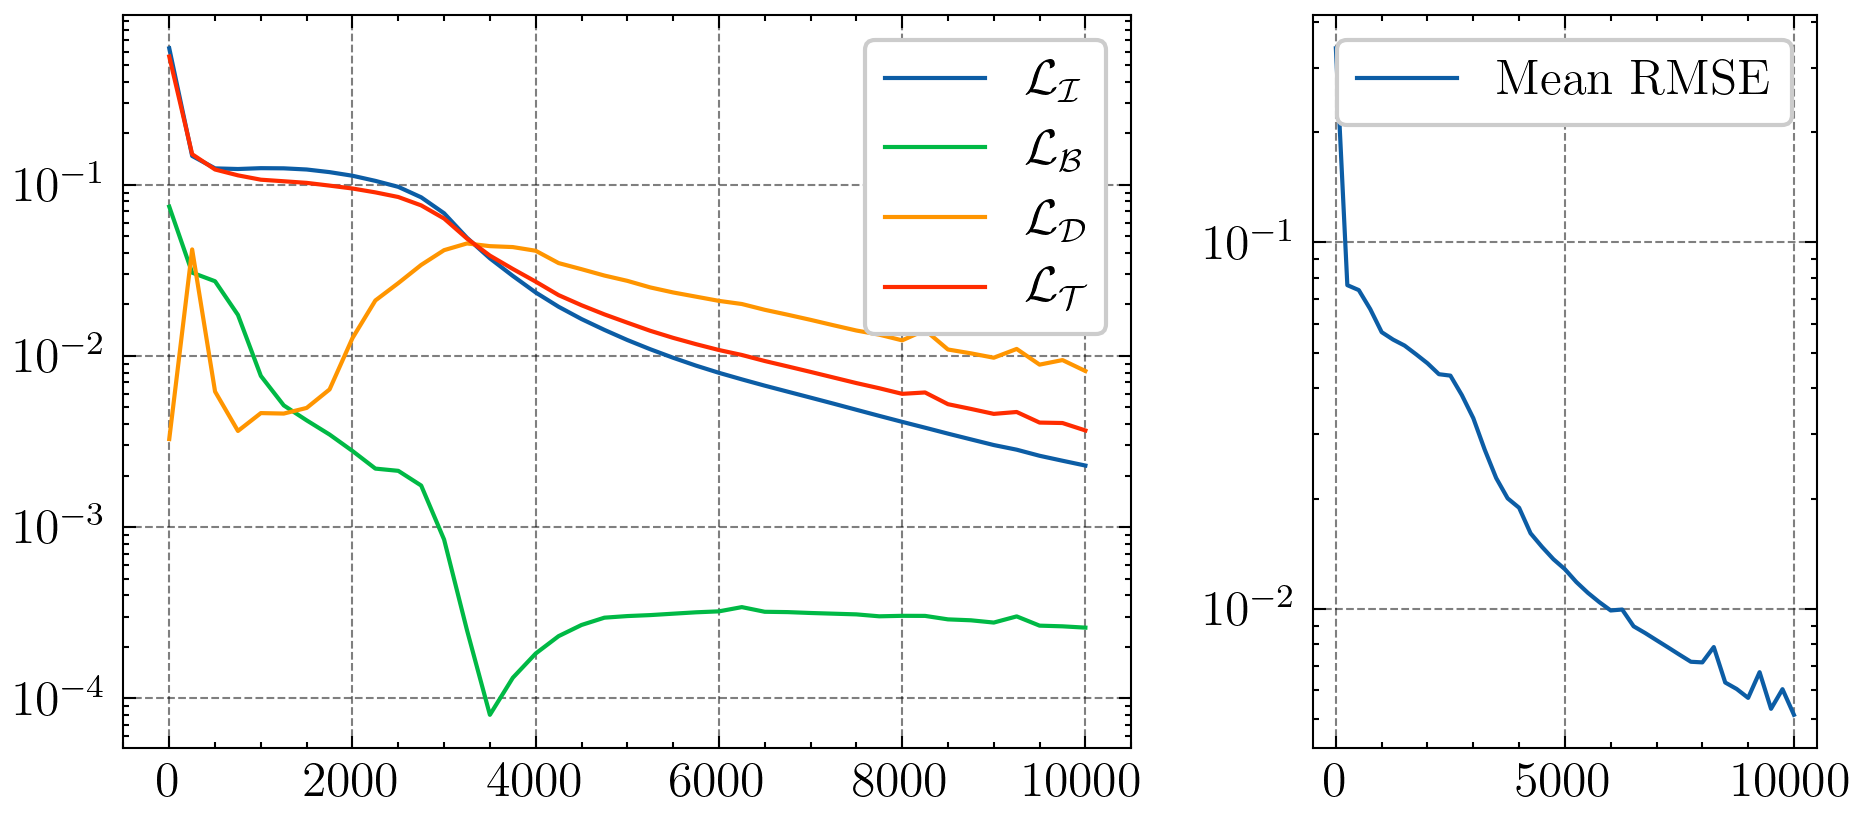
\includegraphics{../images/diffusion/Loss report.png}
    \caption{Динамика функций ошибок для решения уравнения диффузии.}
    \label{fig:diffusion:losses}
\end{figure}

Подробнее о том, как были реализованы PINNs для решения описанных задач, смотрите в приложении \ref{section:appendix:pinn}.

\section{Оценка роли гиперпараметров} \label{section:hyperparameters}

Для анализа этого вопроса нам потребуется ввести две классификации. Разделим переменные нашего сеттинга на три группы:

\begin{enumerate}
    \item Относящиеся к постановке задачи. Это само дифференциальное уравнение, его параметры $\gamma$, а также выбранная область интереса $\Omega$ и соответственно заданные граничные условия. Кроме того, существует несколько типов задания граничных значений, но в нашем случае мы рассматриваем исключительно задачу Коши.
    \item Относящиеся к выбору аппроксимирующей функции и механизму аппроксимации. Это архитектура модели $\mathcal{N}(z; \theta)$, количество слоёв $L$, размер матрицы на каждом слое $W_i$, выбранные функции активации $\nu$, также конкретная реализация использования нейросетевой модели - например, мы можем параметризовать решение следующим образом:
    $$
    \hat{x}(t) \approx x_0 + t \mathcal{N}(t; \theta),
    $$
    и тогда мы автоматически заставляем модель удовлетворять начальному условию $x_0$. То же самое можно сделать для граничных условий, и это называется hard constraint. Тогда мы избавляемся от необходимости минимизировать $\mathcal{L}_B$ и задача оптимизации становится легче. Для наших задач мы будем использовать soft constraint - модель должна сама научиться удовлетворять начальным условиям, и для этого будет введён соответствующий гиперпараметр. Решение, таким образом, представляется в виде
    $$
    \hat{x}(t) \approx \mathcal{N}(t; \theta)
    $$
    \item Относящиеся к процессу обучения. Это выбранное правило оптимизации $O$, соответствующие гиперпараметры - learning rate $lr$, веса функции потерь $\alpha, \beta$, количество итераций $I$, количество точек внутри области $N_\mathcal{F}$.
\end{enumerate}

Это разделение можно выразить так: 1 - какую задачу мы решаем, 2 - чем мы аппроксимируем решение, 3 - как ищем аппроксиматор. Роль каждой переменной, очевидно, различна.

Нашей задачей является минимизация функции потерь относительно параметров $\theta$. Ландшафтом функции потерь мы называем поверхность, задаваемую функцией $\mathcal{L}(\theta) : \mathbb{R}^p \to \mathbb{R}$, и процесс поиска минимума как дискретное движение вдоль этой поверхности. Ландшафт функции потерь - важный элемент в исследовании процесса обучения и оценке обобщающей способности модели \cite{li2018visualizing}, его кривизна влияет на то, как тяжело оптимизатору будет сойтись к минимуму и сможет ли оптимизатор застрять где-то в плохом регионе. В нашем случае на его форму влияют следующие параметры: постановка самой задачи, выбранная архитектура нейросети, а также коэффициенты функции потерь $\alpha, \beta$. Точки коллокации работают как мини-батч и дают приблизительную оценку значения $\mathcal{L}(\theta)$ - чем их больше, тем точнее значение.

Введём также другую классификацию переменных: те, которые влияют на ландшафт потерь, и те, которые не влияют на него. К последним относится алгоритм оптимизации и некоторые его гиперпараметры (lr, weight decay, momentum и т.п.), точки коллокации, количество итераций (эпох), а также конкретный способ использования оптимизатора (например, можно использовать сначала Adam, потом L-BFGS, а можно использовать только один из них; можно реализовать раннюю остановку, а можно подобрать подходящее число итераций; можно по-разному выбирать точку старта и т.д.).

Эти две классификации позволят нам проанализировать роль тех или иных параметров на процесс обучения. Первая классификация более натуральна, когда ставится конкретная задача и необходимо выяснить, какой вклад дают различные элементы в её решение; вторая возникает, когда ставится вопрос об обучении PINNs в принципе, в общем случае. 

\subsection{Влияние гиперпараметров на качество обучения}

\subsection{Влияние размера и инициализации нейросетевой модели}

\subsection{Влияние постановки задачи на оптимальные гиперпараметры}

\section{Анализ сходимости PINNs к решению ДУ} \label{section:errorAnalysis}

\subsection{Теоретические гарантии сходимости}

\subsection{Оценка глобальной погрешности решения}

Простейший способ проанализировать, насколько хорошо работает наше нейросетевое решение - сравнить его с общепринятыми методами численного решения, а ещё лучше - рассмотреть задачи с доступным точным решением. Доверие к нему, таким образом, будет опираться на опыт. Однако существует ряд теоретических методов, которые мы рассмотрим далее.

Возьмём нотацию, описанную в \cite{Cuomo2022}. Пусть $u(z) : \Omega \to X$ - искомая функция, $\mathcal{N}(z; \theta)$ - нейросетевая модель с фиксированной архитектурой. Мы хотим получить оценку величины
$$
\|\mathcal{N}(z; \theta) - u(z)\|,
$$
основываясь на информации об архитектуре модели и тренировочных данных, а также, может быть, на догадках о каких-либо свойствах искомой функции. 

Стоит ещё раз заметить, что функция $\mathcal{N}(z; \theta)$ не определяется единственным образом своими параметрами, а имеет также и архитектуру - конкретный способ реализации параметров. Он может заметно влиять на качество решения и его также необходимо брать в расчёт. Для того, чтобы стандартизовать анализ, можно ввести понятие сложности функции, или её экспрессивности, и выработать способ количественного измерения этой характеристики. Возможно, это позволит упростить методологию.

Пусть дан набор точек $z_i$ и соответствующих значений функции $u(z_i)$, где $i \in \{1, ..., N\}$ (например, это какая-либо совокупность измерений искомого решения ДУ, начальных и граничных условий). Тогда \textit{эмпирический риск} для модели с фиксированными параметрами $\theta$ определяется как
$$
\mathcal{\hat{R}}[\mathcal{N}] = \frac{1}{N}\sum_{i=1}^{N}\|\mathcal{N}(z_i) - u(z_i)\|^2
$$

Общий \textit{риск} модели, характеризующий её способность аппроксимировать функцию на всём $\Omega$, будет определяться как
$$
\mathcal{R}[\mathcal{N}] = \int_{\Omega}(\mathcal{N}(z) - u(z))^2dz
$$

Качество решения можно оценить, исходя из трёх факторов.

\paragraph{Ошибка оптимизации.} Обозначим модель, полученную в результате тренировки, как $\mathcal{N}^*$. Мы введём \textit{ошибку оптимизации} как меру качества тренировочного процесса для данной нейросетевой архитектуры на данных тренировочных точках. Мы ожидаем, что если достигнут минимум ошибки оптимизации, дальнейший способ улучшения качества - поиск новых данных и использование новых архитектур. 

Обычно ошибка оптимизации нам неизвестна на практике, т.к. функция потерь является сильно невыпуклой, а стандартные методы оптимизации дают лишь приближённое решение (нередко застревая в локальном минимуме). Математически она будет выражаться как разница между эмпирическим риском полученной модели $\hat{u}^*$ и наименьшим эмпирическим риском из всех возможных:
$$
\varepsilon_O = \mathcal{\hat{R}}[\mathcal{N}^*] - \inf_{\theta}\mathcal{\hat{R}}[\mathcal{N}]
$$

Равенство $\varepsilon_O = 0$ будет означать, что мы нашли глобальный минимум.

\paragraph{Ошибка аппроксимации.} Введём \textit{ошибку аппроксимации}, описывающую, насколько хорошо мы можем аппроксимировать искомую функцию, используя данную архитектуру. Математически она определяется как наименьший возможный общий риск для данной архитектуры:
$$
\varepsilon_A = \inf_{\theta}\mathcal{R}[\mathcal{N}]
$$

Способность нейросетей аппроксимировать различные классы функций широко изучена в литературе и именно в данном контексте играют роль теоремы универсальной аппроксимации, которые, в сущности, утверждают, что $\epsilon_A$ можно сделать сколь угодно малой при правильном выборе архитектуры модели и количества параметров. Редко, однако, говорится о том, как именно выбирать архитектуру и размер модели - эта область ещё мало изучена, хоть в ней и есть свои результаты.

\paragraph{Ошибка обобщения.} Она характеризует способность нейросети делать верные предсказания на тех данных, которые не встречались в тренировочном наборе. Она выразится как максимальное отклонение общего риска от эмпирического риска при данной архитектуре и данных тренировочных точках:
$$
\varepsilon_G = \sup_{\theta}|\mathcal{R}[\mathcal{N}] - \hat{\mathcal{R}}[\mathcal{N}]|
$$

\section*{Заключение} \label{section:conclusion}
\addcontentsline{toc}{section}{Заключение}

\printbibliography[heading=bibintoc,title={Список источников}]

\appendix

\section{Детали реализации методологии PINN} \label{section:appendix:pinn}

\section{Детали анализа роли гиперпараметров} \label{section:appendix:hyperparameters}

\section{Метод оценки оптимальных гиперпараметров} \label{section:appendix:hpo}

\section{Некоторые наблюдения и соображения} \label{section:appendix:thoughts}

\end{document}